\documentclass{article}\usepackage[]{graphicx}\usepackage[]{color}
%% maxwidth is the original width if it is less than linewidth
%% otherwise use linewidth (to make sure the graphics do not exceed the margin)
\makeatletter
\def\maxwidth{ %
  \ifdim\Gin@nat@width>\linewidth
    \linewidth
  \else
    \Gin@nat@width
  \fi
}
\makeatother

\definecolor{fgcolor}{rgb}{0.345, 0.345, 0.345}
\newcommand{\hlnum}[1]{\textcolor[rgb]{0.686,0.059,0.569}{#1}}%
\newcommand{\hlstr}[1]{\textcolor[rgb]{0.192,0.494,0.8}{#1}}%
\newcommand{\hlcom}[1]{\textcolor[rgb]{0.678,0.584,0.686}{\textit{#1}}}%
\newcommand{\hlopt}[1]{\textcolor[rgb]{0,0,0}{#1}}%
\newcommand{\hlstd}[1]{\textcolor[rgb]{0.345,0.345,0.345}{#1}}%
\newcommand{\hlkwa}[1]{\textcolor[rgb]{0.161,0.373,0.58}{\textbf{#1}}}%
\newcommand{\hlkwb}[1]{\textcolor[rgb]{0.69,0.353,0.396}{#1}}%
\newcommand{\hlkwc}[1]{\textcolor[rgb]{0.333,0.667,0.333}{#1}}%
\newcommand{\hlkwd}[1]{\textcolor[rgb]{0.737,0.353,0.396}{\textbf{#1}}}%

\usepackage{framed}
\makeatletter
\newenvironment{kframe}{%
 \def\at@end@of@kframe{}%
 \ifinner\ifhmode%
  \def\at@end@of@kframe{\end{minipage}}%
  \begin{minipage}{\columnwidth}%
 \fi\fi%
 \def\FrameCommand##1{\hskip\@totalleftmargin \hskip-\fboxsep
 \colorbox{shadecolor}{##1}\hskip-\fboxsep
     % There is no \\@totalrightmargin, so:
     \hskip-\linewidth \hskip-\@totalleftmargin \hskip\columnwidth}%
 \MakeFramed {\advance\hsize-\width
   \@totalleftmargin\z@ \linewidth\hsize
   \@setminipage}}%
 {\par\unskip\endMakeFramed%
 \at@end@of@kframe}
\makeatother

\definecolor{shadecolor}{rgb}{.97, .97, .97}
\definecolor{messagecolor}{rgb}{0, 0, 0}
\definecolor{warningcolor}{rgb}{1, 0, 1}
\definecolor{errorcolor}{rgb}{1, 0, 0}
\newenvironment{knitrout}{}{} % an empty environment to be redefined in TeX

\usepackage{alltt}

\usepackage[utf8x]{inputenc}
\usepackage[francais]{babel}
\usepackage[T1]{fontenc}
\usepackage[autolanguage,np]{numprint}
\usepackage{boxedminipage}

\usepackage{longtable}
\usepackage{rotating} 
\usepackage{supertabular} 
\usepackage{colortbl}

\title{Exhaustivité des données}
\author{Dr J-C. Bartier - RESURAL}
\date{Janvier 2014}
\IfFileExists{upquote.sty}{\usepackage{upquote}}{}

\begin{document}

\maketitle
\begin{abstract}
Ce document compare le nombre de RPU transmis au nombre de passages déclarés au serveur de veille et d'alerte SAGEC.
\end{abstract}




\section{Source des données}

Les données concernant le nombre de passages dans les services d'urgence polyvalents d'Alsace proviennent de deux sources:
\begin{enumerate}
  \item le serveur de veille et d'alerte (SAGEC Alsace) recueille les données des établissements qui possédaient un service d'urgence en 2005 (Wisssembourg, Saverne, Haguenau, HUS, Clinique Saine-Odile, Sélestat, Colmar, Guebwiller, Thann, Alkirch, Clinique des trois frontières). Ces établissements remontent un bulletin quotidien \footnote{moins de 1 an, de 1 à 75 ans, plus de 75 ans, total des passages, UHCD, transferts}. On y ajoute la clinique Sainte-Anne depuis le 1er janvier 2013 qui transmet la même information.
  \item les RPU transmis par douze des quatorze établissements ayant un service d'urgence polyvalent dont les médecins sont des urgentistes (Wisssembourg, Saverne, Haguenau, HUS, Clinique Saine-Odile, Sélestat, Colmar, Guebwiller, Thann, Alkirch, Clinique des trois frontières, Clinique Diaconnat-Fonderie). Cette procédure est active depuis le premier janvier 2013.
\end{enumerate}

Les RPU donnent des informations qui recouvrent toalement celles du serveur régional tout en apportant des informations beaucoup plus complètes et dont la granularité est plus fine. A terme, les informations transmises au serveur de veille devrait disparaitre au profit de la remontée des RPU. Le présent travail essaie de répondre à cette question.

\section{Comparaison des données}

% latex table generated in R 3.0.2 by xtable 1.7-1 package
% Sat Jan 25 17:37:51 2014
\begin{table}[ht]
\centering
\begin{tabular}{rrrrrrrr}
  \hline
 & 3FR & ALK & COL & DIA & GUE & HUS & MUL \\ 
  \hline
SAU & 16423 & 14352 & 64650 & 7078 & 15531 & 121190 & 62806 \\ 
  RPU & 15688 & 7126 & 64758 & 29469 & 15103 & 37018 & 56195 \\ 
   \hline
\end{tabular}
\end{table}
% latex table generated in R 3.0.2 by xtable 1.7-1 package
% Sat Jan 25 17:37:51 2014
\begin{table}[ht]
\centering
\begin{tabular}{rrrrrrrr}
  \hline
 & ODI & SAV & SEL & TAN & WIS & HAG & ANN \\ 
  \hline
SAU & 25675 & 26915 & 18076 & 14704 & 11205 & 0 & 14661 \\ 
  RPU & 25963 & 12424 & 19790 & 0 & 12646 & 34414 & 0 \\ 
   \hline
\end{tabular}
\caption[Comparaisons RPU-Passages]{Comparaison RPU renseignés et Passages (SAU) déclarés en 2013} 
\label{fig:rpu_p}
\end{table}

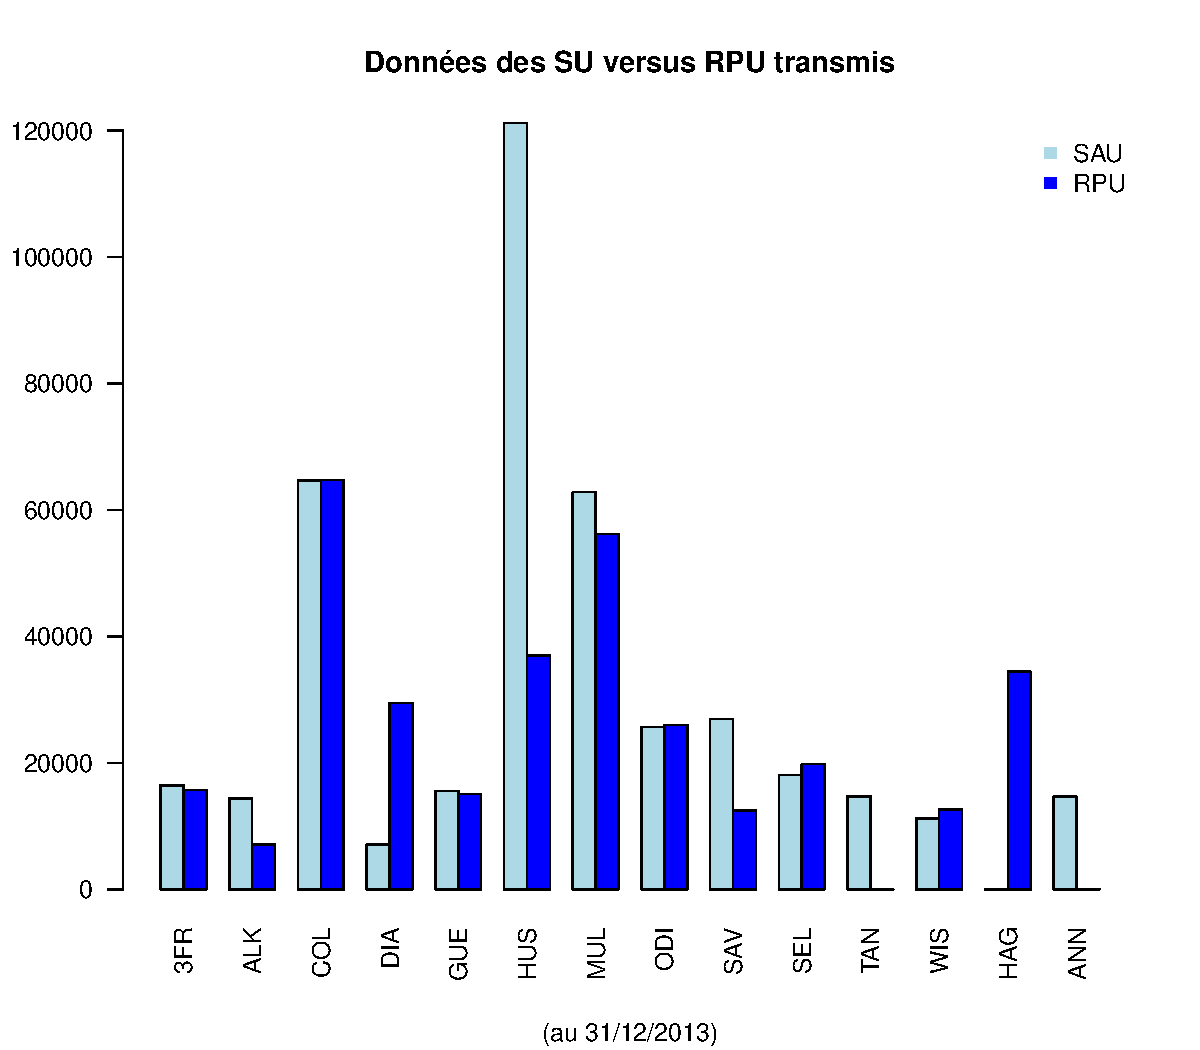
\includegraphics[width=\maxwidth]{figure/sau_rpu} 



\textbf{Remarques:}
\begin{itemize}
  \item \emph{RPU} sont les RPU transmis à e-santé. A terme ce devrait être la seule donnée d'activité recueillie. On remarque pour 2013 qu'on est loin de l'exhaustivité.
  \item \emph{SAU} données d'activité transmise au serveur régional de veille. Ces données sont recueillies depuis 2005 sauf pour trois établissements. Deux d'entre eux (StAnne et Diaconnat fonderie) n'existaient pas en tant que SU au moment de l'implantation du serveur.
  \item Le\emph{CH Haguenau} ne transmet plus au serveur régional depuis plusieurs années.
  \item le \emph{SU Saverne} ne transmets des RPU que depuis fin juillet 2013
  \item le \emph{CH Thann} n'a jamais transmis de RPU
  \item la \emph{Clinique Ste Anne} ne transmet pas de RPU mais transmet des données d'activité quotidienne sur le modèle du serveur régional.
  \item le \emph{CH Sélestat} n'a pas transmis de RPU pendant 3 mois (août à novembre 2013)
  \item le \emph{CH d'Alkirch} n'a pas transmis de RPU pendant les premières semaines de 2013.
\end{itemize}


\begin{center}
\begin{boxedminipage}{10cm}
 \begin{itemize}
  \item nombre total de passages déclarés: $\textbf{413 266}$ 
  \item nombre total de RPU déclarés: \textbf{330 594}
 \end{itemize}
\end{boxedminipage}
\end{center}

Si on suppose que le nombre de passages déclarés est exact (en réalité sous estimé, par ex. Haguenau), l'exhaustivité mesurée est de l'ordre de \textbf{80\%} .

\section{Conclusion}

La comparaison des deux sources de données montre que l'exhaustivité quantitative des RPU est nettement inférieure à celle du serveur régional. Cette situation justifie le maintien du serveur de veille tant que la remontée des RPU n'a pas atteint un niveau équivalent.

\end{document}

